Figure \ref{wpmAGREE} shows an exmaple of direct modelling the component semantics in the AADL AGREE annex. This is mostly done by augumenting the contracts defined in synchronous AGREE, and adding additional contracts to enforce the output hold rule.

\begin{figure}[ht!]
\centering
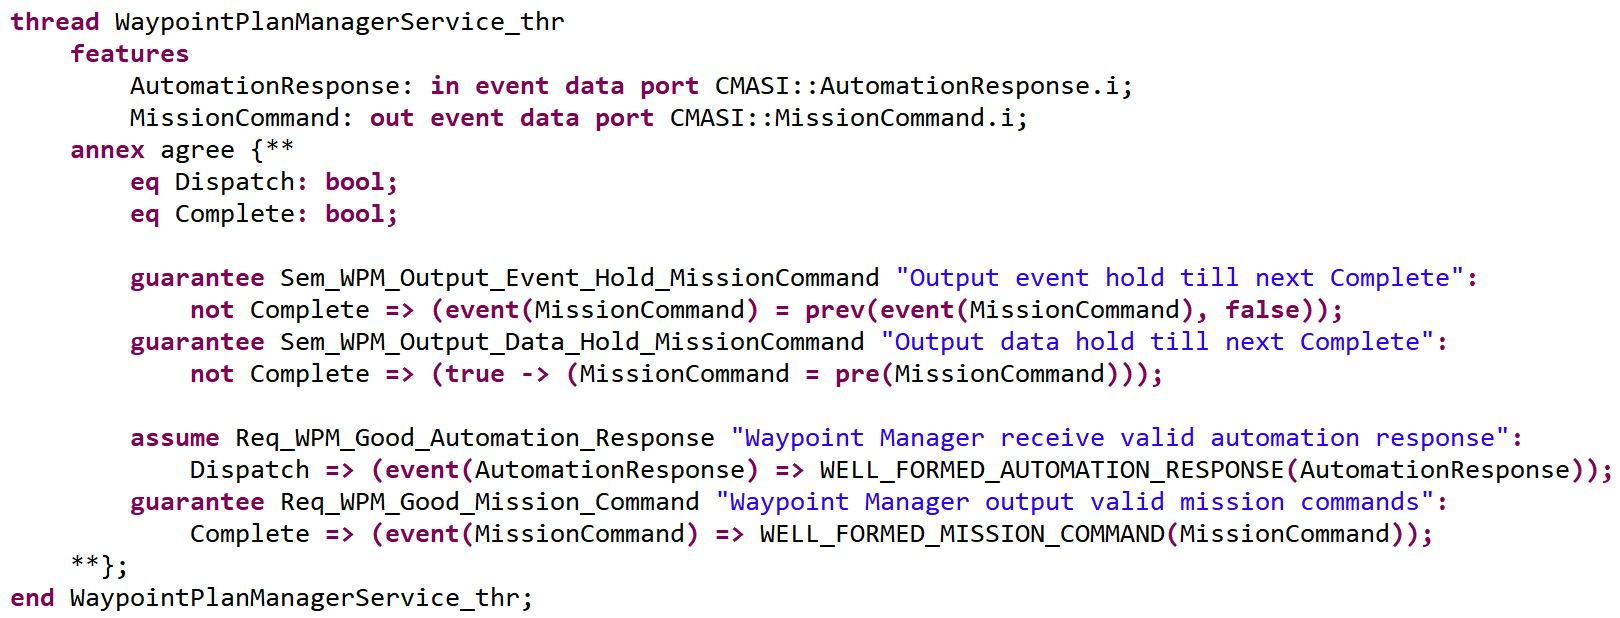
\includegraphics[width=130mm]{wpmAGREE.jpg}
\caption{An AGREE Model Example\label{wpmAGREE}}
\end{figure}

We showed an example of directly modelling the scheduling semantics in AGREE. But for complicated contracts (e.g. involving history), this is not a straightforward task. Thus, we model the scheduling semantics behind the scene during the AGREE translation. We propose a new AGREE usage flow, where a user has to choose the desired MoC (synchronous or scheduled AGREE) under which the contracts are to be verified. The choice of MoC is inspired by the concept of \emph{director} adopted in the Ptolemy project \cite{Ptolemy}. If the scheduled AGREE is chosen, the user also needs to specify a schedule. Currently, we assume a model of the schedule in AGREE is provided. Then, the AGREE translator will generate the corresponding Lustre model reflecting the desired semantics. AGREE uses a variant of Lustre \cite{GAO2008111} language as its backend. It introduced an expression called \emph{condact} to clock nodes, i.e. \emph{Condact (clock, node\_name(), initial\_output)}. It is essential to model the scheduling semantics. A clocked node updates the local and output signals when the clock is true, otherwise it keeps the previous value of the local and output signals. We are aware that more recent Lustre developement introduced similar temporal operators like \emph{when} and \emph{current}. We use \emph{condact} simply because it is supported by the underlying SMT solver.

In AGREE backend, each AADL thread is translated to a Lustre node, as shown in Figure \ref{WPMlustre}. Note that the translation uses a \emph{constraint} style, where thread outputs are mapped to the node inputs. This means that the \emph{condact} expression does not directly clock the thread outputs. We add Lustre assertions to ensure outputs and states hold. Figure \ref{lustreAsync} shows an example of the usage of \emph{condact} with assertions. Note that we use the \emph{complete} event to clock the node. 

\begin{figure}[ht!]
\centering
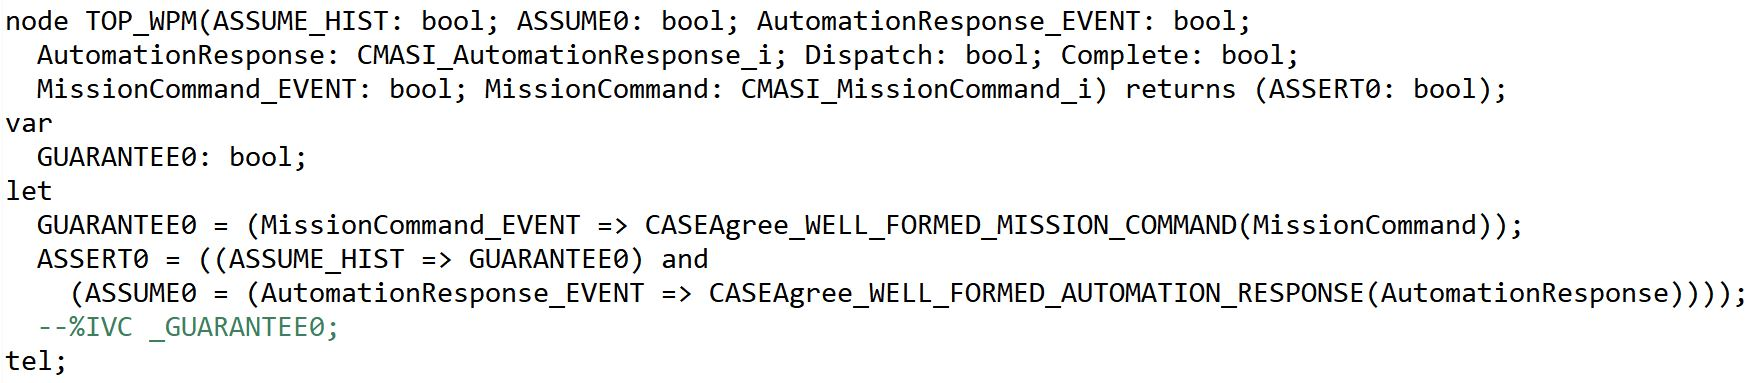
\includegraphics[width=120mm]{wpmLustre2.jpg}
\caption{A Lustre Model of AADL Thread \label{WPMlustre}}
\end{figure}

\begin{figure}[ht!]
\centering
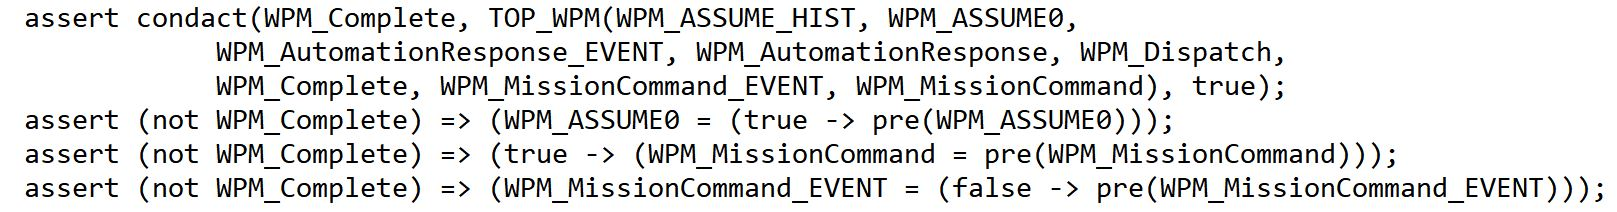
\includegraphics[width=120mm]{lustreAsync4.jpg}
\caption{A Lustre expression \emph{condact} Usage Example\label{lustreAsync}}
\end{figure}

%\begin{figure}[ht!]
%\centering
%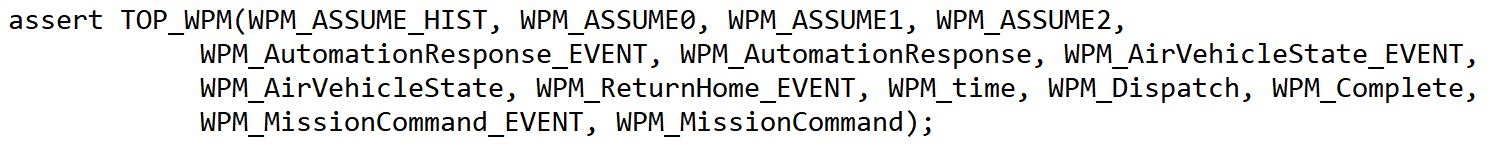
\includegraphics[width=120mm]{lustreSync2.jpg}
%\caption{An AADL Model Illustrating Motivation\label{lustreSync}}
%\end{figure}

%\begin{lstlisting}[language=c,frame=single,caption=An AGREE model of a schedule,label=schedule_model]
%  assert condact(WPM__Complete, _TOP__WPM(WPM____ASSUME__HIST, WPM____ASSUME0, WPM____ASSUME1, WPM____ASSUME2, 
%				WPM__AutomationResponse___EVENT_, WPM__AutomationResponse, WPM__AirVehicleState___EVENT_, WPM__AirVehicleState, 
%                WPM__ReturnHome___EVENT_, WPM__time, WPM__Dispatch, WPM__Complete, WPM__MissionCommand___EVENT_, WPM__MissionCommand), true);
%  assert (not WPM__Complete) => (WPM____ASSUME0 = (true -> pre(WPM____ASSUME0)));
%  assert (not WPM__Complete) => (WPM____ASSUME1 = (true -> pre(WPM____ASSUME1)));
%  assert (not WPM__Complete) => (WPM____ASSUME2 = (true -> pre(WPM____ASSUME2)));
%  assert (not WPM__Complete) => (true -> (WPM__MissionCommand = pre(WPM__MissionCommand)));
%  assert (not WPM__Complete) => (WPM__MissionCommand___EVENT_ = (false -> pre(WPM__MissionCommand___EVENT_)));
%\end{lstlisting}  
  